\chapter{Proposta para análise de arquiteturas de microsserviços \ac{mmorpg}}
\label{cap3}

Para realizar a análise de consumo de recursos de uma arquitetura de jogos \ac{mmorpg} é necessário coletar / medir os recursos utilizados para posterior análise.
%
Na fase de coleta de informação, é possível utilizar ferramentas existentes para coletar informações sobre o consumo da rede (\textit{e.g.}, Tcpdump, Wireshark, etc.) e consumo de recursos computacionais do serviço (e.g., Golang Flame, Ruby Thread profiler tool, Golang profiler, \textit{etc.})
%
Estas ferramentas contribuem com a análise, sendo de extrema importância para a coleta de dados.
%
Este tópico será abordado na Seção~ref{sec:metricas}.



Contudo, se faz necessário uma arquitetura de microsserviços para jogos \ac{mmorpg} a fim de ser utilizado para análise.
%
Esta arquitetura será descrita na Seção~\ref{sec:arquitetura_proposta}.


\section{Ferramentas de análise de consumo de recursos}
\label{sec:metricas}


Para efetuar a análise de uma arquitetura, de faz necessário um sistema de monitoramento a fim de obter métricas do uso de recursos do sistema.
%
Para este fim, se faz necessário obter três classes de aplicação:


\begin{enumerate}
  \item Banco de dados para métricas
  \item Sistema de alimentação do banco de dados
  \item Sistema de visualização do banco de dados
\end{enumerate}

Nesse sentido, se faz necessário obter um banco de dados específico ao armazenamento de métricas.
%
O banco \textit{Graphite}\footnote{Graphite: \url{https://github.com/graphite-project}} é específico a esta operação.
%
Ele permite o envio de registros utilizando texto plano por chamadas de sistema, \ac{udp} ou \ac{tcp}.
%
Um exemplo de chamada de sistema pode ser visualizado na Figura~\ref{fig:graphite}.

\begin{figure}[htb!]
  \caption{Inserindo dados no Graphite utilizando chamada de sistema.}
  \label{fig:graphite}
  \begin{lstlisting}[language=bash]
    # Exemplo de chamada de sistema em Bash
    $ echo "foo.bar 1 `date +%s`" | nc localhost 2003
  \end{lstlisting}
  \centering

  Fonte:~\cite{graphite}.
\end{figure}

Para visualização dos dados, o sistema \textit{web Grafana}\footnote{Grafana: \url{https://github.com/grafana/}} exibe os dados armazenados pelo \textit{Graphite} em um \textit{dashboard}.
%
Este \textit{dashboard} pode ser visualizado na Figura~\ref{fig:grafana}.


\begin{figure}[htb!]
  \caption{Dashboard de análise do Grafana.}
  \label{fig:grafana}
  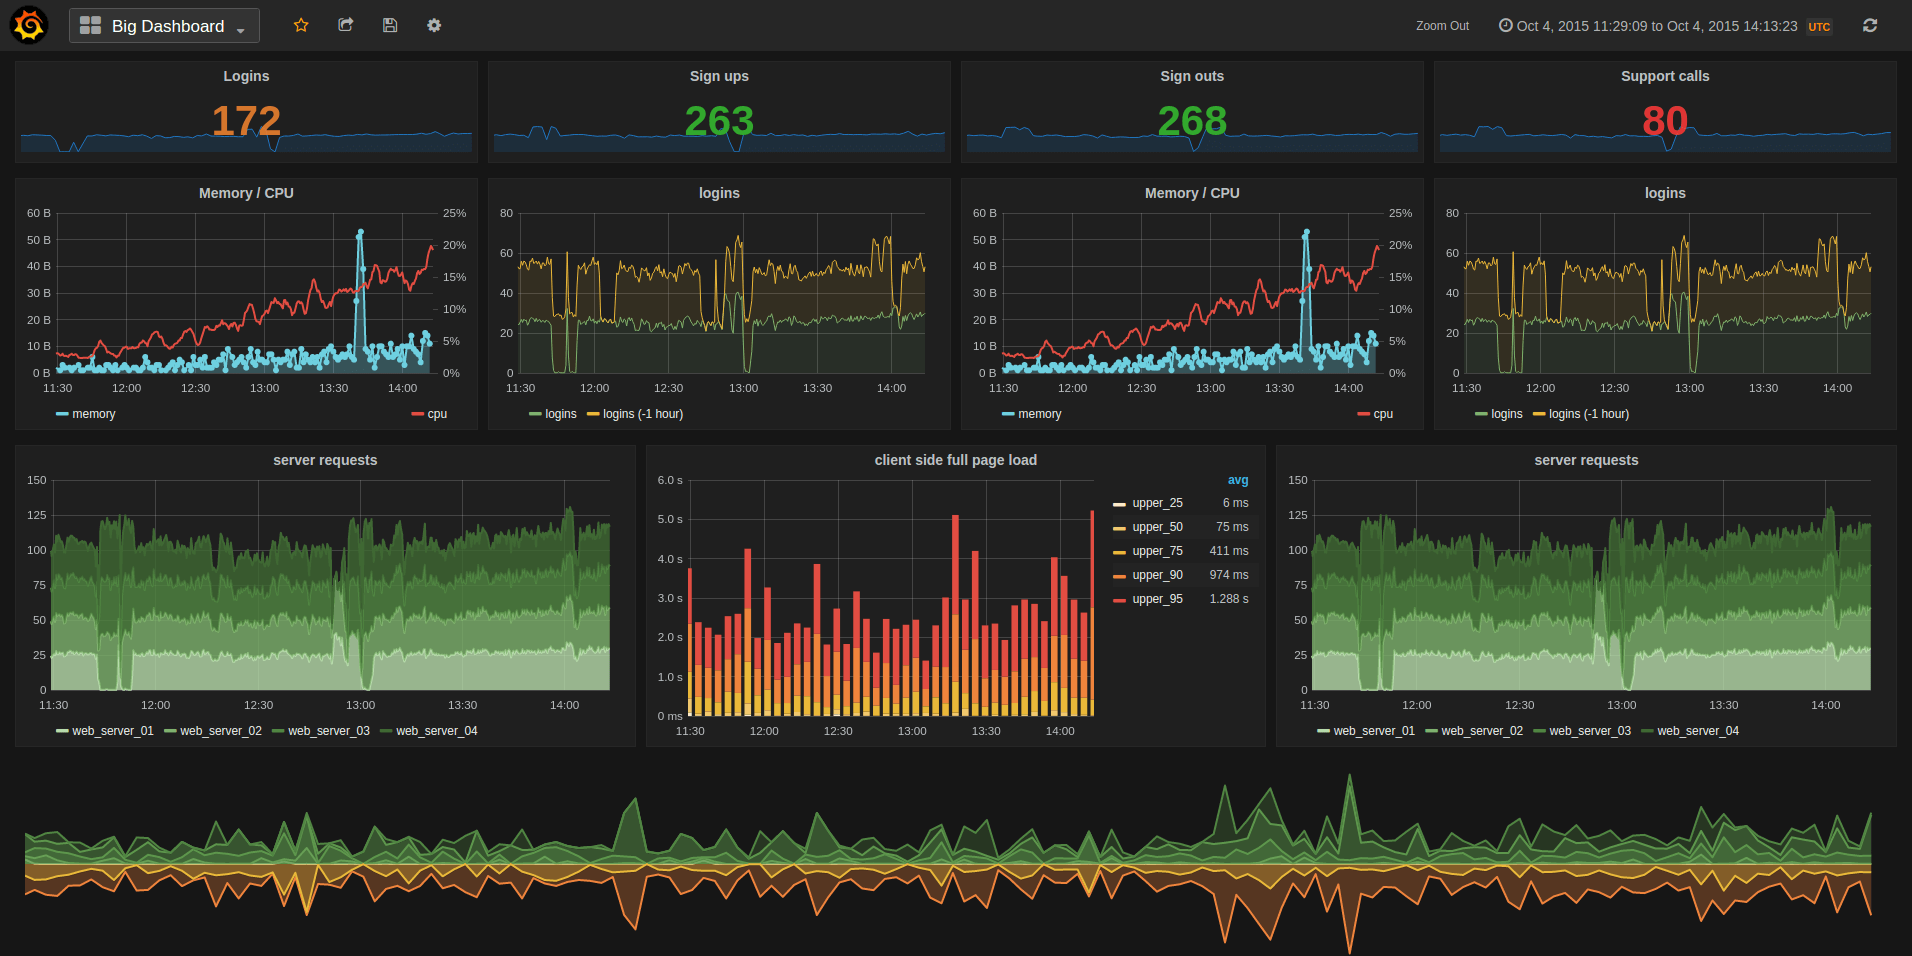
\includegraphics[height=5cm]{img/cap3/grafana.png}
  \centering

  Fonte:~\cite{grafana}.
\end{figure}

Entretanto, se faz necessário o envio de métricas de uso de recursos pelos próprios microsserviços.
%
Nesse sentidio, ferramentas de análise (\textit{e.g.}, TCPDump, Go Pprofit, etc.) e informações do sistema operacional serão utilizadas para popular o banco de dados.
%
A Figura~\ref{fig:estatistica} informa o funcionamento do serviço que receberá as métricas dos microsserviços.


\begin{figure}[htb!]
  \caption{Dashboard de análise do Grafana.}
  \label{fig:estatistica}
  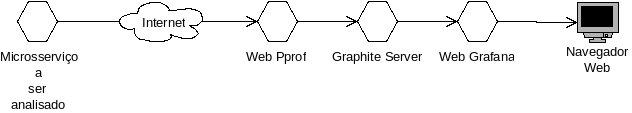
\includegraphics[height=3cm]{img/cap3/estrutura_de_estatistica.png}
  \centering

  Fonte:~\cite{grafana}.
\end{figure}


O microsserviço \textit{Web Pprof} exibido na Figura~\ref{fig:estatistica} receberá requisições web com os seguintes parâmetros:


\begin{enumerate}
  \item \textit{service\_id}: Referenciará qual microsserviço é o emissor desta requisição.
  \item \textit{service\_hash}: Servirá para autenticar a requisição do microsserviço.
  \item \textit{service\_ram}: Valor de ponto flutuante que indicará a memória consumida, em Megabytes.
  \item \textit{service\_bw}: Valor de ponto flutuante que indicará a o consumo de banda pelo serviço, em Megabytes.
  \item \textit{service\_disk}: Valor de ponto flutuante que indicará o consumo de disco, em Gigabytes.
\end{enumerate}

Com estes parâmetros, será possível analisar o consumo de recursos e custo de operação da arquitetura analisada.
%
Entretanto, faz necessário simular esta arquitetura.
%
Nesse sentido, a descrição da arquitetura analisada é importante, a fim de descrever sua funcionalidade para que se comporte igual a uma arquitetura de microsserviços para jogos \ac{mmorpg}.



\section{Arquitetura proposta para análise}
\label{sec:arquitetura_proposta}



Esta seção tem como objetivo descrever a arquitetura implementada para análise, baseada na arquitetura Salz~\cite{albion_online_unite}.
%
A mesma arquitetura é utilizada no jogo Sandbox-Interactive Albion\footnote{Sandbox-Interactive Albion: \url{https://albiononline.com/en/home}}.
%
Ela pode ser vista em uma visão macro na Figura~\ref{fig:salz}.



\begin{figure}[htb!]
\caption{Arquitetura de microsserviços proposta para análise.}
\label{fig:salz}
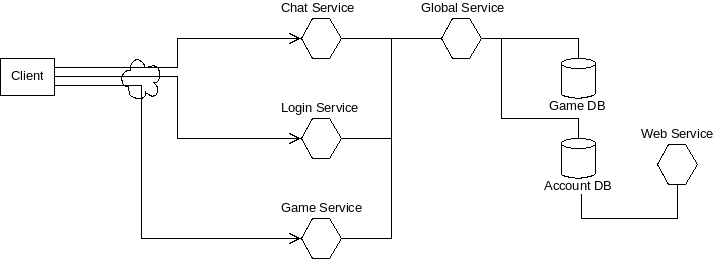
\includegraphics[height=5cm]{img/cap3/salz.png}
\centering

Adaptado de:~\cite{albion_online_unite}.
\end{figure}


Todos os elementos descritos na Figura~\ref{fig:salz} são microsserviços, e por este motivo devem funcionar de forma independente dos demais serviços.
%
Essa arquitetura contém os seguintes microsserviços:

\begin{itemize}
  \item \textbf{Login Service}: Responsável por gerenciar as conexões do jogo e fornecer autorização aos clientes para os demais microsserviços.
  \item \textbf{Chat Service}: Receberá mensagens e distribuirá aos demais jogadores da mesma região ou enviará mensagens diretas a outros jogadores. Ele receberá a conexão diretamente do jogador, e por sua vez será necessário utilizar a tecnologia \ac{jwt} assinado pelo serviço \textit{Login Service} para autenticar a conexão.
  \item \textbf{Game Service}: Gerenciará um pedaço do ambiente do jogo. Cada microsserviço desta categoria será responsável por um pedaço de ambiente do jogo, na qual controlará as ações dos personagens em relação a sua área de interesse. Ele receberá a conexão diretamente do cliente, e por sua vez usará a mesma técnica de autenticação do \textit{Chat Service} para autenticar a conexão.
  \item \textbf{Global Service}: Este microsserviço resolve as requisições globais requisitadas pelo \textit{chat service}, \textit{login service} ou \textit{game service}. Será responsável por orquestrar os microsserviços, gerenciar as mudanças de microsserviços dos clientes e obter métricas referentes ao jogo, como número de personagens, ações principais e coordenação geral do jogo. Além disso, ele será o gerente de operações \ac{crud} ao banco de dados \textit{Account DB}.
  \item \textbf{Web Service}: Servirá para gerênciar o banco de dados utilizando operações~\ac{crud}.
  \item \textbf{Game DB}: Banco de dados em memória utilizado pelos microsserviços para compartilhamento do estado de mundo.
  \item \textbf{Account DB}: Banco de dados persistente para armazenar o estado de jogo em disco.
\end{itemize}


Para melhor compreendimento se faz necessário a descrição específica de funcionamento em cada microsserviço, tecnologias e protocolos utilizados e esquema de funcionamento.



\subsection{Login Service}



O microsserviço respoonsável por efetuar a autenticação do usuário aos demais microsserviços é nomeado \textit{Login Service}, descrito na Figura~\ref{fig:login_service}.
%
Ele será responsável por impedir multiplas conexões utilizando um mesmo usuário, e assinar um token que será utilizado para autenticação nos demais microsserviços.



\begin{figure}[htb!]
\caption{\textit{Login Service}}
\label{fig:login_service}
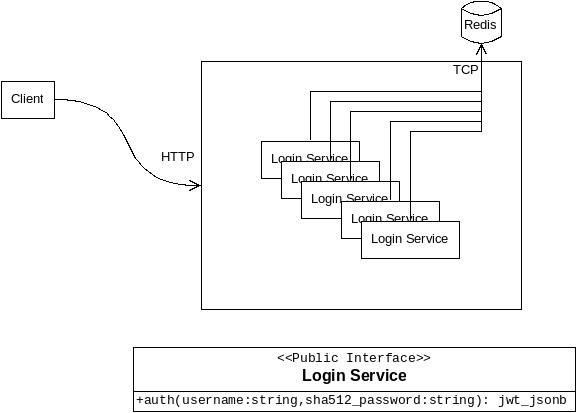
\includegraphics[height=10cm]{img/cap3/login_service.png}
\centering

Elaborado pelo autor.
\end{figure}



Além dessa funcionalidade, outro objetivo deste microsserviço é descrever o status de conexão de um jogador, a fim de sinalizar os demais microsserviços que o mesmo desconectou do serviço.
%
Ele será o responsável pela descrição de status da atual conexão do jogador com o serviço visto que os demais microsserviços estão trabalhando de forma isolada.
%
Isto servirá para evitar requisições maliciosas ao serviço.
%
Nesse sentido, faz necessário que o \textit{Login Service} comunique frequentemente os demais serviços de interesse para que atualize o status de conexão dos jogadores e suas credenciais de conexão, além de obrigar ao cliente uma requisição em um espaço determinado de tempo.



Este microsserviço usará Redis, um banco NoSQL baseado em chave-valor de armazenamento em memória para armazenar tokens de autenticação de uma conexão.
%
Para gerar este token, será utilizado a tecnologia \ac{jwt}, a fim que permita a assinatura de dados pelo serviço de autenticação e a validação nos demais microsserviços que tem interface pública na rede.



\subsection{Chat Service}


Este microsserviço será responsável por redirecionar mensagens a jogadores, e pode ser visualizado na Figura~\ref{fig:chat_service}.


\begin{figure}[htb!]
  \caption{\textit{Chat Service}}
  \label{fig:chat_service}
  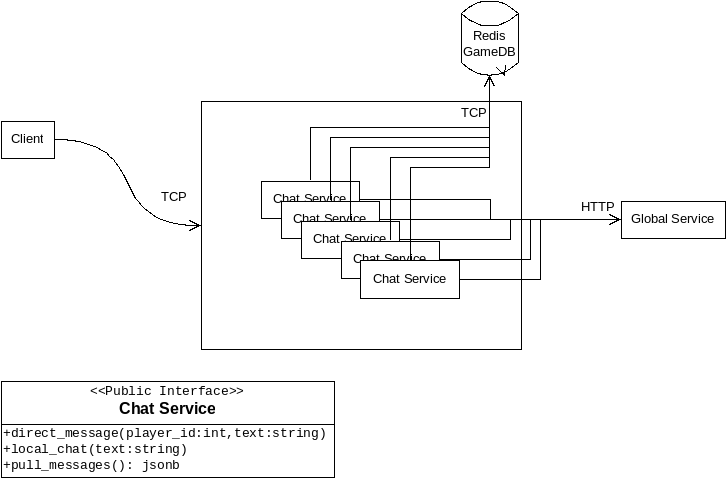
\includegraphics[height=10cm]{img/cap3/chat_service.png}
  \centering

  Elaborado pelo autor.
\end{figure}


Este serviço terá três principais funções na interface pública:



\begin{itemize}
  \item \textit{local\_chat}: Envia mensagens aos personagens que estão na área de interesse do remetente.
  \item \textit{direct\_message}: Envia mensagens diretas a outros personagens.
  \item \textit{pull\_messages}: Recebe mensagens não lidas até então.
\end{itemize}


Para compartilhamento de informações do ambiente de jogo, o microsserviço terá acesso ao GameDB a fim de obter informações de posicionamento dos personagens.
%
Entretanto, a abordagem para mensagens diretas é mais complexa.
%
Se faz necessário o redirecionamento das mensagens entre microsserviços a fim de entregar ao microsserviço onde o destinatário esteja conectado.
%
Para este redirecionamento funcionar, será necessário uma tabela de localização da conexão deste jogador, a qual armazenará a relação entre o personagem e o IP:Porta do microsserviço a qual ele está conectado.
%
Por este motivo, o microsserviço terá acesso ao \textit{GameDB}.
%
No mesmo sentido, mensagens a jogadores offline não são entregues com roteamento, sendo necessário o armazenamento para entrega posterior, tendo esta requisição armazenada junto ao \textit{Global Service}.



\subsection{Game Service}



Este microsserviço gerenciará conexões de uma determinada região do ambiente do jogo, nomeado \textit{chunk}.
%
Ele servirá para atualizar a árvore de cena do cliente e executar operações sobre a árvore de cena do chunk a qual o serviço ficou responsável.
%
A abordagem de divisão em \textit{chunks} serve para minimizar a influência de conexões sobre as operações no mundo, e assim permitir mais conexões sobre um único mundo compartilhado.
%
Entretando é necessário tomar uma abordagem para definir a troca de contexto entre duas \textit{chunks} no jogo.
%
Neste microsserviço foi escolhida a abordagem sobre banco de dados~\cite{albion_online_unite}, onde o cliente terá que trocar de microsserviço conforme a sua localidade a troca de mapa e armazenar estra troca de dados no banco para que o microsserviço que controla esta região possa resgatar seus dados e prosseguir com o jogo.



\subsection{Global Service}

Este microsserviço realizará o meio de campo entre todos os microsserviços.
%
Ele será responsável por sincronizar as posições dos personagens entre o Chat Service e Game Service, atualizar informações do GameService no AccountDB além de gerenciar o GameDB.
%
Ele é uma aplicação \textit{Web} e pode ser um gargalo na aplicação.

\subsection{Web Service}

Este microsserviço será responsável por exibir dados do banco aos jogadores.
%
No contexto de simulação ele servirá para realizar operações \ac{crud} manuais e automatizadas no banco, além de gerenciar migrações no mesmo.

\subsection{GameDB}

\subsection{AccountDB}
